\chapter{印刷简史}
\label{chap:printing}

\begin{quotation}
Printing is a human achievement that has demonstrated far greater power to shape the world than all the forces of mordern weaponry.
\begin{flushright}
    --- John F. Kennedy
\end{flushright}
\end{quotation}

人类和其他动物的差别之一是语言和文字,而语言文字使得知识的记载、积累和传承成为可能。印刷的出现促进了大规模知识传播,是人类文明史上的里程碑。

一般而言,印刷 (printing) 包含四种要素:印版 (image carrier) 、印刷材料、墨、印刷设备;以及两大过程:排版 (typesetting) 和压印 (presswork)。排版负责转换原始的图像和文字,在印版上制作印纹;而压印则负责给印纹上墨,在印刷材料上印制出图文。有时人们会把压印和印刷这两个词混用,我们姑且认为广义的印刷包括排版和狭义的印刷。

当然以上只是一种笼统概括的说法。比如打印机并没有印版,至少没有物理印版。但是我们可以认为图像输出到打印机之前,在电脑内是以虚拟印版的形式存在的。也就是说打印机达到了“机中无版,心中有版”的境界。

窃以为印版是印刷的核心,而数字电脑的应用是印刷工业的一个分水岭,所以下面分四个部分 (传统印刷、传统排版、数字印刷、数字排版) ,按印刷排版技术发展的大致顺序对它们作简单介绍。这里主要谈印版和排版,略谈打印机,基本不涉及印刷材料、墨、印刷机等,因为这些议题和 \LaTeX 关系太远。

\section{传统印刷}
传统印刷按过程和和方法可以分为四大类:

\begin{enumerate}
    \item 凸版印刷 (relief printing) ,印纹凸出印版,凸纹表面上墨,压印到印刷材料上。包括雕版 (block) 、活字 (moveble type) 、活版 (letterpress)、柔版 (flexography) 等技术。
    \item 凹版印刷 (intaglio printing) ,印纹部分凹下,凹纹中灌墨。包括雕刻 (engraving) 、针刻 (drypoint) 、磨刻 (mezzotint) 、蚀刻 (etching)、细点蚀刻 (aquatint)  等方法。
    \item 平版印刷 (planography) ,印纹和非印纹部分在同一个平面上,利用油水相斥原理或感光材料上墨。包括石版 (lithography) 、石版胶印 (offset lithography) 等技术。
    \item 孔版印刷 (porous printing) ,印版上有孔,油墨从其中渗漏到印刷材料上。包括镂空 (stenciling) 、丝网印刷 (screen-printing) 等方法。
\end{enumerate}

\subsection{凸版印刷}

雕版可以追溯到东汉末年,也就是公元220年以前。当时工匠们把文字和图形雕刻在整块木版上,然后涂上墨或染料,再印到丝织品或布料上。木版的缺点是易磨损而难修改。隋唐年间,雕版印刷一度盛行。现存最早的雕版印刷品是唐代868年的《金刚经》 (\autoref{fig:jingangjing}) 。 \footnote{原藏于敦煌莫高窟,1907年被英国考古学家Marc A. Stein (1862--1943) 盗走,现存于大英博物馆。}

\begin{figure}[htbp]
\centering
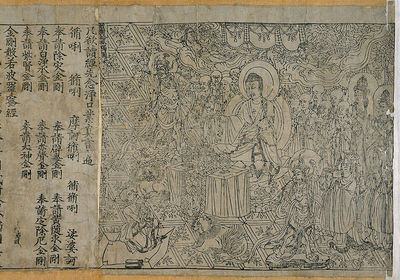
\includegraphics[width=350pt]{jingangjing_sm.jpg}
\caption{《金刚经》,雕版,868}
\label{fig:jingangjing}
\end{figure}

北宋宝元年间,湖北印刷工毕升 (970--1051)\indexBiSheng{} 在1040年左右发明了活字印刷术。他用胶泥刻字,火烧成陶;然后将活字排入铁版,整版印刷。其后在中国和朝鲜都曾出现过金属活字。

活字印刷术后来经由俄罗斯和阿拉伯传入欧洲。在东方技术的影响下,德国出版家Johannes Gutenberg (1398--1468)\indexGutenberg{} 于1450年前后发明了活版印刷术,包括铅字、油墨和印刷机 (printing press) 等技术。

Gutenberg同学用油墨取代了水墨,使得印刷品更耐久。传说他年轻时做过金匠,拥有丰富的金属材料知识,因而顺理成章地发明了合金铅字。这种铅字比木、陶、铜材料的活字都更耐用,印刷效果也更清晰;缺点是它含有铅、锡、锑等有害金属,流毒甚广。这个故事告诉我们,在人类文明的历史上,发展和环保总是一对矛盾。

这些技术迅速推动了西方社会科技文化的发展,导致了文艺复兴。\autoref{fig:bible} 是Gutenberg在1455年印制的《圣经》 \footnote{图中拷贝现存于美国国会图书馆。}。

\begin{figure}[htbp]
\centering
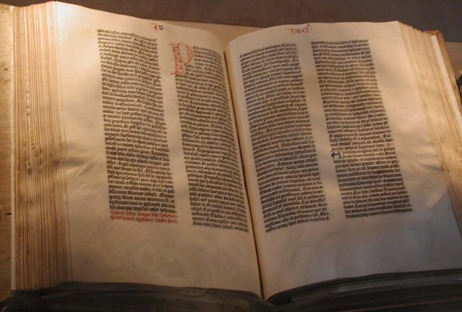
\includegraphics[width=350pt]{gutenberg_bible_sm.jpg}
\caption{Gutenberg Bible, letterpress, 1455}
\label{fig:bible}
\end{figure}

19世纪末出现了柔性版印刷,它使用柔软的橡胶或聚合物材料作印刷版,可以使用几乎所有印刷材料,包括塑料、金属薄膜、玻璃纸等特殊材料。柔性版常用于印刷产品包装。

\subsection{凹版印刷}

凹版印刷一般用铜制印版,也有用锌、铁的,多用于版画。15世纪中叶,雕刻凹版出现于德国和意大利,它用刻刀在印版上刻画比较直的线条。针刻也是15世纪发源于德国,它用带有针状尖端的工具在印版上刻画。\autoref{fig:durer} 是德国艺术家Albrecht Dürer (1471--1528)\indexDurer{} 的雕刻作品《圣克里斯托弗》 \footnote{克里斯托弗是天主教和东正教的圣徒,传说身高六米,面目狰狞。某日他驼一小儿渡河,及其半渡,河水暴涨,小儿体沉似铅。至彼岸,克氏抱怨:未料汝体重至斯,吾几丧小儿胯下。那小儿正色道:彼时尔肩上是整个世界及其造物主,朕乃自有永有万王之王的耶稣基督。话毕,消弥于无形。}。\autoref{fig:ury} 是德国印象派画家Lesser Ury (1861--1931)\indexUry{} 的针刻作品《咖啡馆中的女人》。

\begin{figure}[htbp]
\centering
\begin{minipage}[t]{0.42\textwidth}
\centering
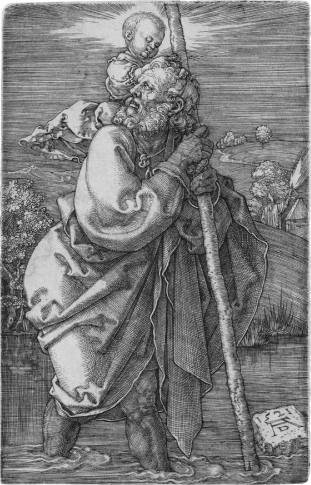
\includegraphics[height=230pt]{durer_st_christopher.jpg}
\caption{St. Christopher, engraving by Dürer, 1521}
\label{fig:durer}
\end{minipage}
\hspace{5pt}
\begin{minipage}[t]{0.48\textwidth}
\centering
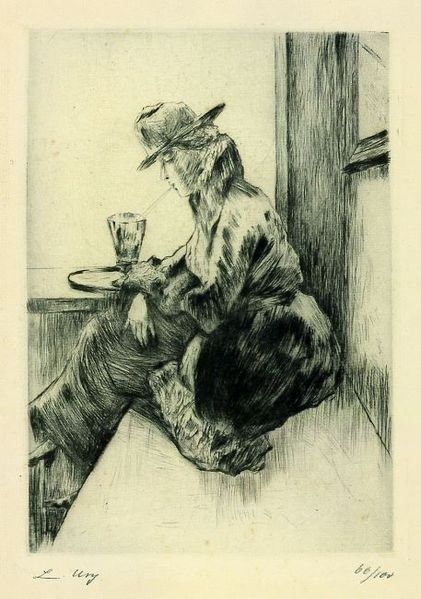
\includegraphics[height=230pt]{ury_woman_in_cafe.jpg}
\caption{Woman in Cafe, drypoint by Lesser Ury}
\label{fig:ury}
\end{minipage}
\end{figure}

15世纪末,德国艺术家Daniel Hopfer (1470--1536)\indexHopfer{} 发明了蚀刻法。先用针在印版上刻画,再用强酸腐蚀印版。\autoref{fig:hopfer}是Hopfer的蚀刻作品《士兵和他的妻子》。

1642年,德国艺术家Ludwig von Siegen (1609--1680)\indexVonSiegen{} 发明了磨刻。先用特制的工具在印版上刮磨出无数微细芒刺,再用刮刀把芒刺作不同程度的刮除,从而获得不同明暗的色调。\autoref{fig:gainsborough} 是一幅19世纪的磨刻仿制作品《乔治亚娜·卡文迪许,德文郡公爵夫人》,原作是英国肖像画家Thomas Gainsborough (1727--1788)\indexGainsborough{} 的同名油画。

\begin{figure}[htbp]
\centering
\begin{minipage}[t]{0.42\textwidth}
\centering
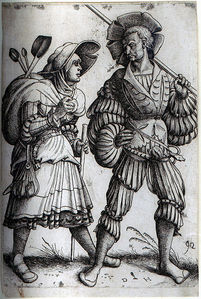
\includegraphics[height=220pt]{hopfer_soldier_wife_sm.jpg}
\caption{The Soldier and his Wife, etching by Hopfer, 1500}
\label{fig:hopfer}
\end{minipage}
\hspace{5pt}
\begin{minipage}[t]{0.48\textwidth}
\centering
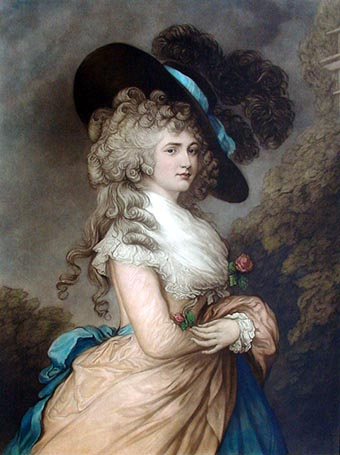
\includegraphics[height=220pt]{gainsborough_georgiana_duchess.jpg}
\caption{Georgiana Cavendish, Duchess of Devonshire, mezzotint}
\label{fig:gainsborough}
\end{minipage}
\end{figure}

细点蚀刻则在印版上洒一层薄薄的树脂粉,加热使之把粘附于版面。酸在树脂微粒间渗入,把版面腐蚀出大量小坑,坑中装墨。这样印制的版画有水粉画的效果,其色调纹理取决于酸的强度和腐蚀时间。

针刻和细点蚀刻可以结合使用。\autoref{fig:goya} 是西班牙浪漫主义画家Francisco Goya (1746--1828)\indexGoya{} 的雕刻、针刻和细点蚀刻结合作品《理性沉睡,心魔生焉》。\autoref{fig:cassatt} 是美国画家Mary S. Cassatt (1844--1926)\indexCassatt{} 的针刻和细点蚀刻结合作品《浴室》。

\begin{figure}[htbp]
\centering
\begin{minipage}[t]{0.42\textwidth}
\centering
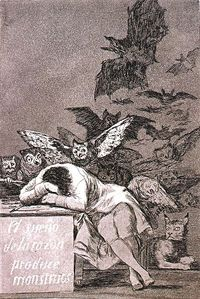
\includegraphics[height=230pt]{goya_sleep_of_reason_sm.jpg}
\caption{Sleep of Reason Produces Monsters, etching, aquatint, and drypoint by Goya, 1799}
\label{fig:goya}
\end{minipage}
\hspace{5pt}
\begin{minipage}[t]{0.48\textwidth}
\centering
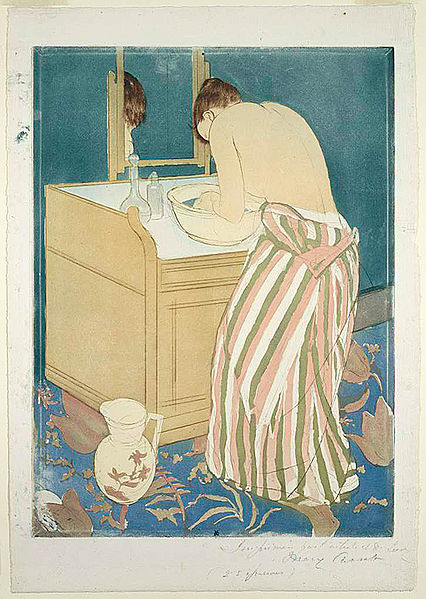
\includegraphics[height=230pt]{cassatt_bath.jpg}
\caption{The Bath, drypoint and aquatint by Cassatt, 1890}
\label{fig:cassatt}
\end{minipage}
\end{figure}

\subsection{平版印刷}

凸版和凹版印刷的压印都是暴力的物理过程,所以印版日久天长会磨损。1796年,德国演员和剧作家Alois Senefelder (1771--1834)\indexSenefelder{} 发明了石版印刷。它利用油和水的互斥性,先用油基材料在光滑的石灰石 (limestone) 版上绘制印纹;再涂上阿拉伯树胶,此胶只会留在无印纹部分;然后把油墨和水的混合物涂在石版上,水附着于无印纹部分,油墨附着于印纹部分。石版印刷利用了简单的化学原理,印版本身在印刷过程中磨损很小。

上述凸版、凹版和平版的压印过程中,印版和印刷材料都直接接触。英国作家Robert Barclay (1648--1690)\indexBarclay{} 和美国印刷工Ira W. Rubel\indexRubel{}分别于1875年和1904年发明了胶印 (offset press) 技术。它先把印版上的图像转移 (offset) 到橡胶布 (rubber blanket) 上,再印到印刷材料上。平版和胶印结合起来的平版胶印效果更清晰,因为橡胶布和印刷材料接触得更充分;印版寿命更长,因为脏活儿累活儿都让橡胶兄弟干了;大批量印刷成本低廉。

1950年代之后,平版胶印逐渐成为应用最广泛的商业印刷技术。而凸版、凹版因为能在印刷品上产生纹路,也还保有一席之地;凸版常用于贺卡、信封、名片、请帖、版画等;凹版常用于钞票、邮票、护照等。

\subsection{孔版印刷}

早在八世纪,勤劳勇敢的中国人民就在印刷过程中使用了镂空方法。它常用于印制纺织品或指示牌上重复的符号、标志、形状、图案。从镂空发展而来的丝网印刷则出现于宋代。丝网印刷可以使用十分广泛的印刷材料,常用于纺织品、产品标签、气球、印刷电路板、医疗设备等。

\section{传统排版}

\subsection{手工排版}

Gutenberg在1450年就发明了印刷机,然而排版还是基本靠手。西文只有几十个字母,加上标点符号也没多少。早年间金属活字装在上下两个带格子的盒子 (job case) 里,大写字母放在上面的盒子 (upper case) 里,小写字母放在 (lower case) 。活字在英文里是type,排版就是typeset,排版工人则是typesetter。排版工人用单个字母排成单词,单词排成行,很多行捆在一起就是一页的印模 (forme) ;印模装到印刷机上。

中文比较麻烦,常用汉字有几千个,光是装活字就得要一个很大的盘子。我猜这也是近代中国科技落后的一个原因,你想,印刷排版落后书籍就少,书籍少人们的文化知识就少。

元大德年间,宣州旌德县令王祯 (1271--1368)\indexWangZhen{} 发明了转轮排字盘。用轻质木材作成一个大轮盘,直径约七尺,轮轴高三尺,轮盘装在轮轴上可以自由转动。把木活字按古代韵书的分类法,分别放入盘内一个个格子里。他做了两副这样的大轮盘,排字工人坐在两副轮盘之间,转动轮盘即可找字,所谓“以字就人,按韵取字”。这样既提高了排字效率,又减轻了排字工的体力劳动,是排字技术上的一个创举。

大德二年 (1298年) ,王祯造三万余木活字,排印《旌德县志》100部,历时一月。1313年,著成13万字的《王祯农书》,主要讲述农业生产技术。术后杂录部分记载了和农业关系不大的“造活字印书法”,其中有转轮排字盘的插图 (见本书封面) 。

\begin{comment}
\begin{figure}[htbp]
\centering
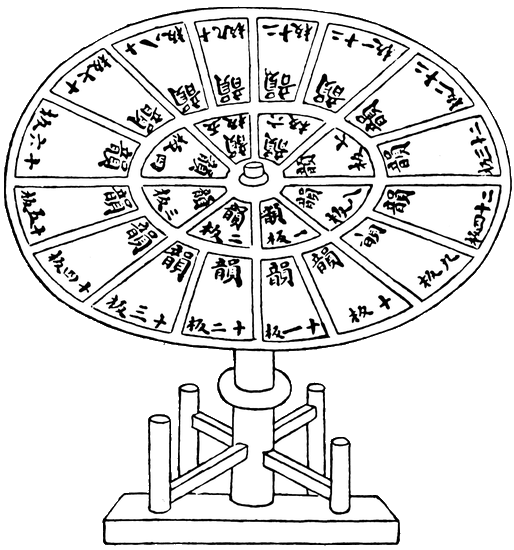
\includegraphics[width=300pt]{movable_type_transparent.png}
\caption{转轮排字盘}
\label{fig:wang}
\end{figure}
\end{comment}

\subsection{机械排版}

直到19世纪末期,机械排版技术才姗姗来迟。排版的机械化和压印的机械化相差了400多年,这充分说明排版和压印的难易程度相去甚远。

1869年,德国商人Karl Kastenbein\indexKastenbein{}发明了键盘排字机,后被英国《泰晤士报》采用。1870年,俄国排版工Peter Kniagininski\indexKniagininski{}在圣彼得堡展出了他的排版机,遗憾的是无人喝彩。他最终酗酒而死。

19世纪末期出现的铸字排版 (hot metal typesetting,hot type) 技术使得排版的效率又上了一个台阶。它用机械的方法把熔化的专用合金注入模具,铸成活字。

1884年,人称古腾堡第二的德裔美人Ottmar Mergenthaler (1854--1899)\indexMergenthaler{} 发明了林诺行式铸排机 (Linotype) ,两年后成立了摩根泰勒林诺铸排机公司 (Mergenthaler Linotype Company)\indexLinotype{}。它用键盘调用活字模具,将其排成一行,整体铸造;效率高,成本低,主要用于报纸印刷。

1885年,美国公务员Tolbert Lanston (1844--1913)\indexLanston{} 发明了莫诺单字铸排机 (Monotype) ,两年后成立了兰斯顿莫诺铸排机公司 (Lanston Monotype Machine Company)\indexMonotypeLanston{}。它用键盘制作穿孔纸带,以纸带驱动搜索活字模具,铸成活字,然后排列成行。单字铸排比行式铸排灵活,纸带可以重用,主要用于书籍印刷。

1897年,匈牙利人C. Méray Horváth\indexMerayHorvath{}发明了远程排版 (teletypography) 技术。它用键盘或打字机发出电报信号来控制不同地点的铸排机。1930年代,《泰晤士报》采用了类似的技术。

1914年,国际排版机公司 (International Typesetting Machine Company)\indexInternationaltype{} 的因特行式铸排机 (Intertype) 上市。林诺机部件多是铸铁材料,而因特机一般用钢和铝。从此排版机领域三足鼎立。

1936年莫诺公司 (Monotype Corp.)\indexMonotype{} 在伦敦股票交易所上市;1999年被比利时的爱克发-吉华集团 (Agfa-Gevaert) 收购;2004年被转卖给美国私募公司塔克·安东尼 (TA Associate),并改组为莫诺图像 (Monotype Imaging)\indexMonotypeImaging 。

1990年林诺公司与西门子\indexSiemens{}的子公司地狱 (Hell) \footnote{1929年德国发明家Rudolf Hell (1901--2002) 创建了该公司,1981年被西门子收购。}合并为林诺-地狱 (Linotype-Hell AG),1997年被海德堡印刷机械 (Heidelberg Printing Machines AG) 收购,其业务被拆分为字体和相关软件,以及排版两部分,前者在2007年被转卖给莫诺图像。

1916年国际排版机公司被改组为因特铸排机公司 (Intertype Corp.)\indexIntertype{},1957年与哈瑞斯公司 (Harris Corp.) 合并。1960年代后机械排版逐渐被照相排版取代,哈瑞斯的业务遂转向通信和信息技术。

\subsection{照相排版}

从1450年到19世纪末期的400多年间,活版印刷在大批量文字的印刷中占据着垄断地位。在这段时期,printing这个词和letterpress是同义的。图文混杂的书籍通常需要两道工序,凹版或石版印制图像,活版印制文字。

而照相排版 (phototypesetting,cold type) 技术的出现打破了这种藩篱。它利用照相感光原理在印版上制作印纹;相应的机器称为照排机 (phototypesetter) 。照相排版可以用于凸版、凹版和平版。

1879年捷克画家Karl Klíč (1841--1926)\indexKlic{} 发明了照相凹版 (photogravure)。在铜版上涂感光胶,曝光后蚀刻。照相凹版比之前的凹版技术质量高,可以产生细腻的纹理和连续的色调。

1946年,因特铸排的照相排版机 (Intertype Fotosetter) 上市,被美国政府印刷局 (U.S. Government Printing Office) 采用。1947年,仙童相机仪器 (Fairchild Camera and Instrument)\indexFairchild{} \footnote{1957年改组为仙童半导体 (Fairchild Semiconductor)。}推出了照相蚀刻机 (photo-engraving machine) 。

以上这些照排机被称为第一代照排机。后来的照排机增加了少许机械电子设备,比如键盘、穿孔纸带等,这就是第二代照排机。1954年,法国人René A. Higonnet (1902--1983)\indexHigonnet{} 和Louis M. Moyroud (1914--2010)\indexMoyroud{} 发明了电子照排机Photon 100。

\section{数字印刷}
数字电脑出现后,打印机应运而生,它们将电脑输出的数字图像转移到打印材料上。比起传统印刷技术,数字印刷成本低,应用方便,也较少浪费化学原料。主要的打印技术有:

\begin{itemize}
    \item 光电打印机 (photoelectric printer) ,利用光电效应 (photoelectric effect) 产生静电摄取墨粉打印到纸上。按光源可以分为是激光打印机 (laser printer) 、发光二极管打印机 (LED printer) 、液晶快门打印机 (LCS printer) 等。
    \item 喷墨打印机 (liquid inkjet printer) ,将墨滴喷到纸张上,通过墨滴的大小来控制图像的浓淡色彩。
    \item 撞击式打印机 (impact printers) ,用打印头 (print head) 撞击色带 (ink ribbon) ,透过色带在纸上留下图像。包括行式打印机 (line printer) 、针式打印机 (dot matrix printer) 。
    \item 热学打印机 (thermal printer) ,利用热学原理,包括直接加热特殊热敏纸的热敏打印机 (direct thermal printer) ,熔化蜡质墨的热蜡传递打印机 (thermal wax transfer printer) ,以及升华染料的热升华打印机 (dye-sublimation printer) 等。
    \item 绘图仪 (plotter) ,控制移动笔来画出矢量图。
\end{itemize}

\subsection{光电打印机}

1930年代,Chester F. Carlson (1906--1968)\indexCarlson{} 在纽约打工时 \footnote{1930年从加州理工物理系毕业后,加入贝尔实验室。1933年大萧条时被解雇,流落到一家专利事务所。一年后跳槽到一家电池公司马洛瑞 (Mallory),也就是后来的金霸王 (Duracell),主持该公司专利部。1936年始在夜校念法律,三年后获法学学士。},需要复制大量专利文件。他觉得光电导性也许可以用于复印:有些材料受到光照时其导电性会改变,静电可以吸附粉末,如果这些粉末是墨粉的话,就可以复制文件。

1938年,Carlson发明了静电复印 (xerography) ,四年后获得专利。但是在他企图商业化这项技术时,几十个公司和政府部门都无动于衷,最后一家从事照相器材的小公司哈罗德 (Haloid Photographic Company)\indexHaloid{} 觉得可以试一试。1959年,哈罗德推出了第一款复印机Xerox 914,1961年公司改名为施乐 (Xerox)\indexXerox{}。

1969年,施乐的Gary K. Starkweather (1938--)\indexStarkweather{} \footnote{1960年密歇根州立大学物理学士,1966年罗彻斯特光学硕士。1964年加入施乐,1988年跳槽至苹果,1997年跳至微软。} 在静电复印技术的基础上发明了激光打印机。激光束照射硒鼓 (selenium drum) ,干墨粉就会被静电吸附。1976年,IBM\indexIBM{}推出了第一款商用激光打印机IBM 3800,体积庞大。第一款办公室用激光打印机是1981年的施乐Star 8010,价格昂贵。1984年惠普\indexHP{}推出了第一款面向大众市场的激光打印机LaserJet。

LED打印机和LCS打印机 \footnote{常被误称为LCD打印机,但是LCD的含义是液晶显示 (liquid crystal display) 。} 分别用发光二极管 (light-emitting diode, LED) 和液晶快门 (liquid crystal shutter, LCS) 作为光源。比起一般的激光打印机,它们运动部件少,因而省电、可靠、便宜,打印速度也较快;缺点是分辨率较低。

1985年,卡西欧\indexCasio{}推出了第一款LCS打印机LCS-2400。同年,冲电气\indexOki{}推出了LED打印机OPP-6220 \footnote{传说LED打印机是卡西欧发明的,但是卡西欧网站公司历史部分只提到了LCS打印机;另传说冲电气1983年就发明了LED打印机,但是冲电气的三个网站都没提及,这三个网站最早的关于LED打印机的记录分别是1985, 1987, 1989年。}。

\subsection{喷墨打印机}

1951年,西门子\indexSiemens{}推出了第一款连续式 (continuous) 喷墨打印机。它用高压泵喷射墨滴并形成静电场,少数墨滴印到纸上,多数被回收重用。它的优点是打印速度快,喷头不会堵塞;缺点是墨水会蒸发,容易浪费。

1977年,西门子推出了可控式 (drop-on-demand) 喷墨打印机。它只在需要时才喷射,比连续式省墨、分辨率高、成本低;只是打印速度较慢。可控式的墨滴在印上纸张前需要一个加压过程,佳能\indexCanon{}、惠普\indexHP{}、Lexmark\indexLexmark{}都用加热的方法汽化墨水来增压,所以被称为热可控式 (thermal DOD) ;爱普生\indexEpson{}则用压电材料 (piezoelectric material) 把电能转化为机械能来增压,所以被称为压电可控式。压电可控式喷墨打印机因为压电材料的原因打印头成本较高,墨水成本较低,常见于商业或工业应用。

1988年惠普推出的DeskJet标志着喷墨打印机走向了大众市场。目前喷墨打印机在家用市场上占据着主导地位。

\subsection{撞击式打印机}

最早的行式打印机出现于1950年代初期,它一次可以打出一行字,配合大型主机使用。字符装在一个鼓上的称为鼓式打印机 (drum printer) ,字符装在一条链上的称为链式打印机 (chain printer) 。链式较容易维护更换零件。1952年的IBM 716是最流行的鼓式打印机,1959年的IBM 1403是最流行的行式打印机。

Unix的两个命令 \texttt{lp} 和 \texttt{lpr} 就来自行式打印机,后来其他一些操作系统也把它们的打印设备或端口命名为 \texttt{LP} 或 \texttt{LPT},不管那打印机到底是不是行式。

针式打印机打印头上的多个针头构成一个点阵 (dot matrix) ,工作时这些针头透过色带在纸上打点组成字符,打印头从左往右移动就打出一行,打完一行后打印头复位;纸张向上移动,就能打出一页。其工作方式类似打字机,只是打字机打出的是字符。

1970年,DEC\indexDEC{}推出了第一款针式打印机LA30,它可以打印80列字符,每个字符由5x7的点阵构成。打印头用步进电机驱动,进纸用齿轮螺杆机构实现。

1980年的爱普生MX-80发起了针式打印机对个人电脑市场的冲锋。1980年代中期,爱普生的LQ系列把打印头针数从增加到24个,能够更好地打印东亚字符,速度也更快。

针式打印机的因为噪音大、速度慢、分辨率低,1990年代之后逐渐被喷墨打印机取代,但是仍然保留在少数场合,比如收银机、票据机、自动柜员机等。

\subsection{热学打印机}

1970年代出现的热敏打印技术,将特殊热敏纸张加热以获取图像,常用于传真机。1976冲电气推出了第一款基于热敏打印的传真机OKIFAX 7100。直到1990年代,多数传真机还在使用热敏打印,后被热蜡打印取代。热敏打印也常见于一些医疗器械,比如超声波仪。它的一个缺点是时间长了字迹会变淡。

热蜡转移打印机将熔化的蜡质墨喷到印鼓上,然后印到纸上,常用于标签、条形码的打印。1940年代佐藤公司\indexSATO{}发明了这项技术。1982年,几家日本公司推出了热蜡转移打印机。

热升华打印机将染料快速加热升华到气态,然后扩散到纸上,常用于照片打印。1980年代末期,杜邦\indexDupont{}推出了热升华打印技术,当时还十分昂贵。1995年法戈电子 (Fargo Electronics)\indexFargo{} \footnote{2006年被休格斯国际 (HIG Global) 收购。}推出了廉价的热升华打印机FotoFun!。

\subsection{绘图仪}

绘图仪主要用于电脑辅助设计 (computer-aided design, CAD) 。早期的绘图仪输出的是矢量图,其他打印设备输出的是点阵图。制图时,画笔横向移动,纸张纵向进给,其工作方式类似数控机床。

1959年,加州电脑技术公司 (Calcomp Technology)\indexCalcomp{} \footnote{1986年被洛克希德收购,1999年解体。} 推出了最早的绘图仪Calcomp 565。1981年,惠普推出了便携式绘图仪HP 7470。

随着喷墨打印机和激光打印机分辨率的提高,电脑内存和速度的发展,矢量图可以在电脑端完成点阵化,然后输出到绘图设备。因此笔式绘图仪逐渐被淘汰。

\section{数字排版}

1963年,Alphanumeric\indexAlphanumeric{}推出了第一个电脑照排系统 \footnote{德国人声称Rudolf Hell发明的Digiset才是第一个电脑照排系统,据说他还发明了电视、传真机、扫描仪。} APS 2,它以DEC PDP 8作为前端,还配有阴极射线管 (cathode ray tube, CRT) ;后来它的前端换为IBM 360。这种武装了电脑技术的第三代照排机很快将铸排机赶出了历史舞台。

但是这种电脑照排机只能一个字一个字地排版,效率还是比较低。1976,莫诺公司推出了第一款激光照排机 (laser imagesetter) Monotype Lasercomp。它用光栅图像处理器 (raster image processor, RIP) 生成点阵图像,再用激光把图像曝光到胶片上,一次可以输出整页。

激光照排机被称为第四代 (也就是最后一代) 照排机 \footnote{按北大方正的说法,王选 (1937--2006) 院士从1975年就开始研发激光照排技术,算是这个领域的先知。遗憾的是文革期间在家养病十年的王老已经不够犀利,直到1988年才推出中国第一台激光照排机。},它采用电脑到胶片 (computer-to-film, CTF) 的技术路线。与之对应的是电脑到印版 (computer-to-plate, CTP) ,相应的设备称为直接制版机 (platesetter) 。这种方法省略了胶片,直接制作印版。1988年,Printware公司\indexPrintware{}推出了第一款直接制版机。

不管是CTF还是CTP,都需要RIP。RIP和它前面的流程放到 \ref{sec:digital_typesetting}节中介绍,因为他们和 \TeX 的关系比较紧密。
